\chapter{Ergebnisse}


\begin{figure}[ht]
    \centering
    \begin{subfigure}[b]{0.35\textwidth}
        \centering
        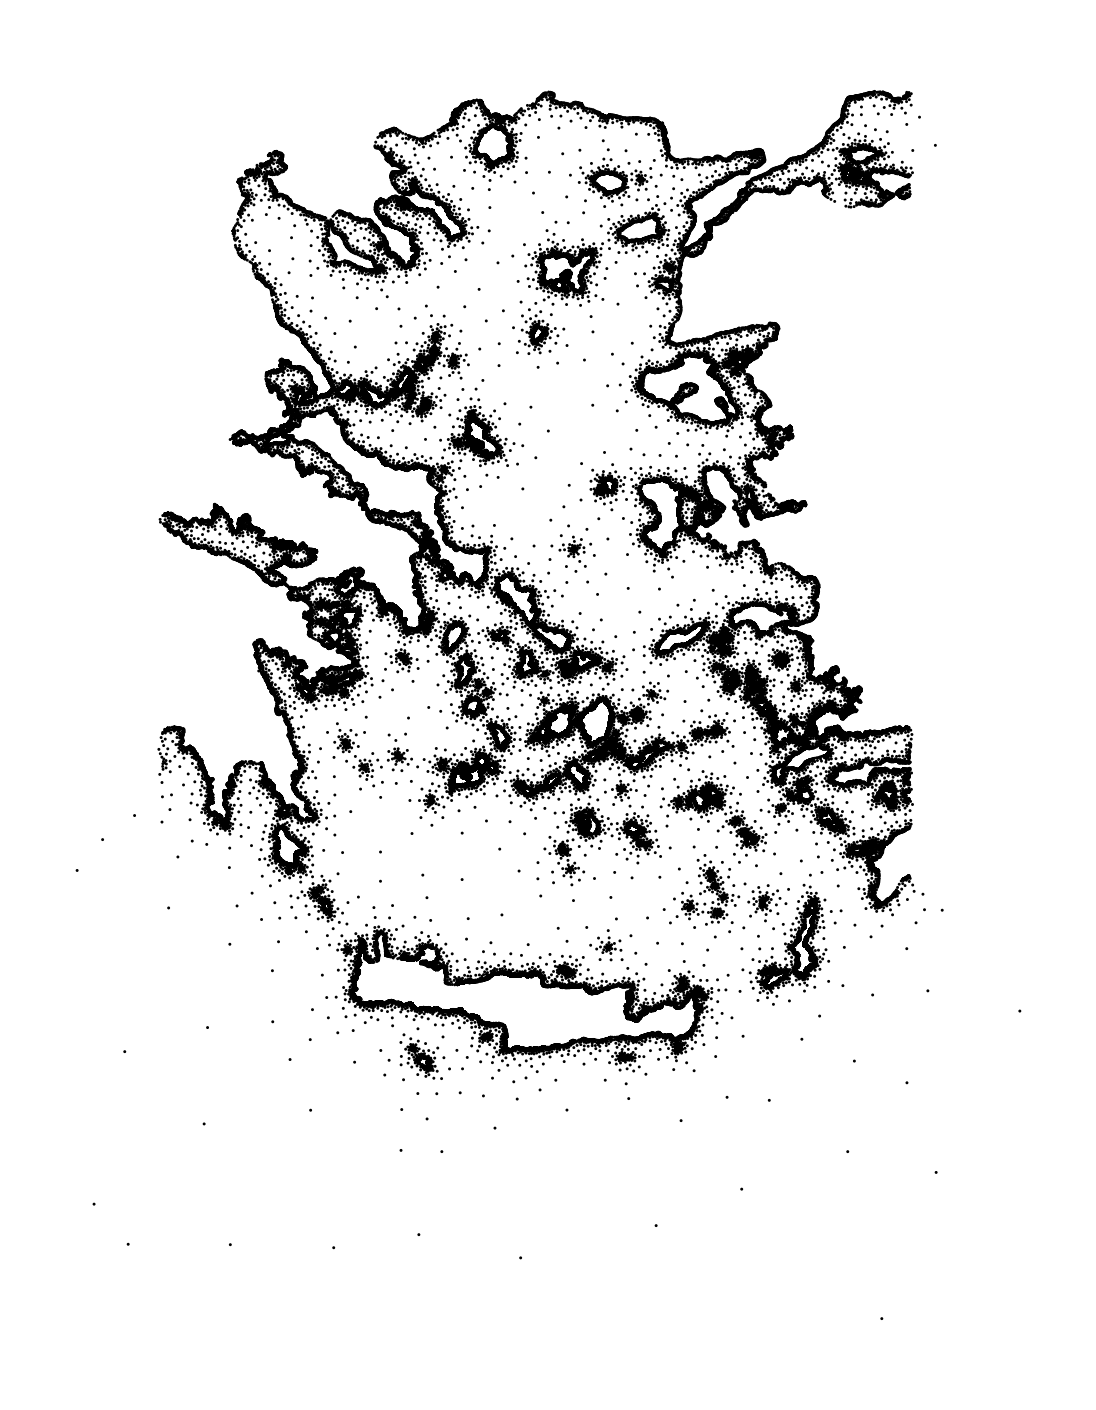
\includegraphics[width=\textwidth]{img/base_graphs/aegaeis-ref-graph.png}
        \caption{aegaeis-graph}
    \end{subfigure}
    \hfill
    \begin{subfigure}[b]{0.35\textwidth}
        \centering
        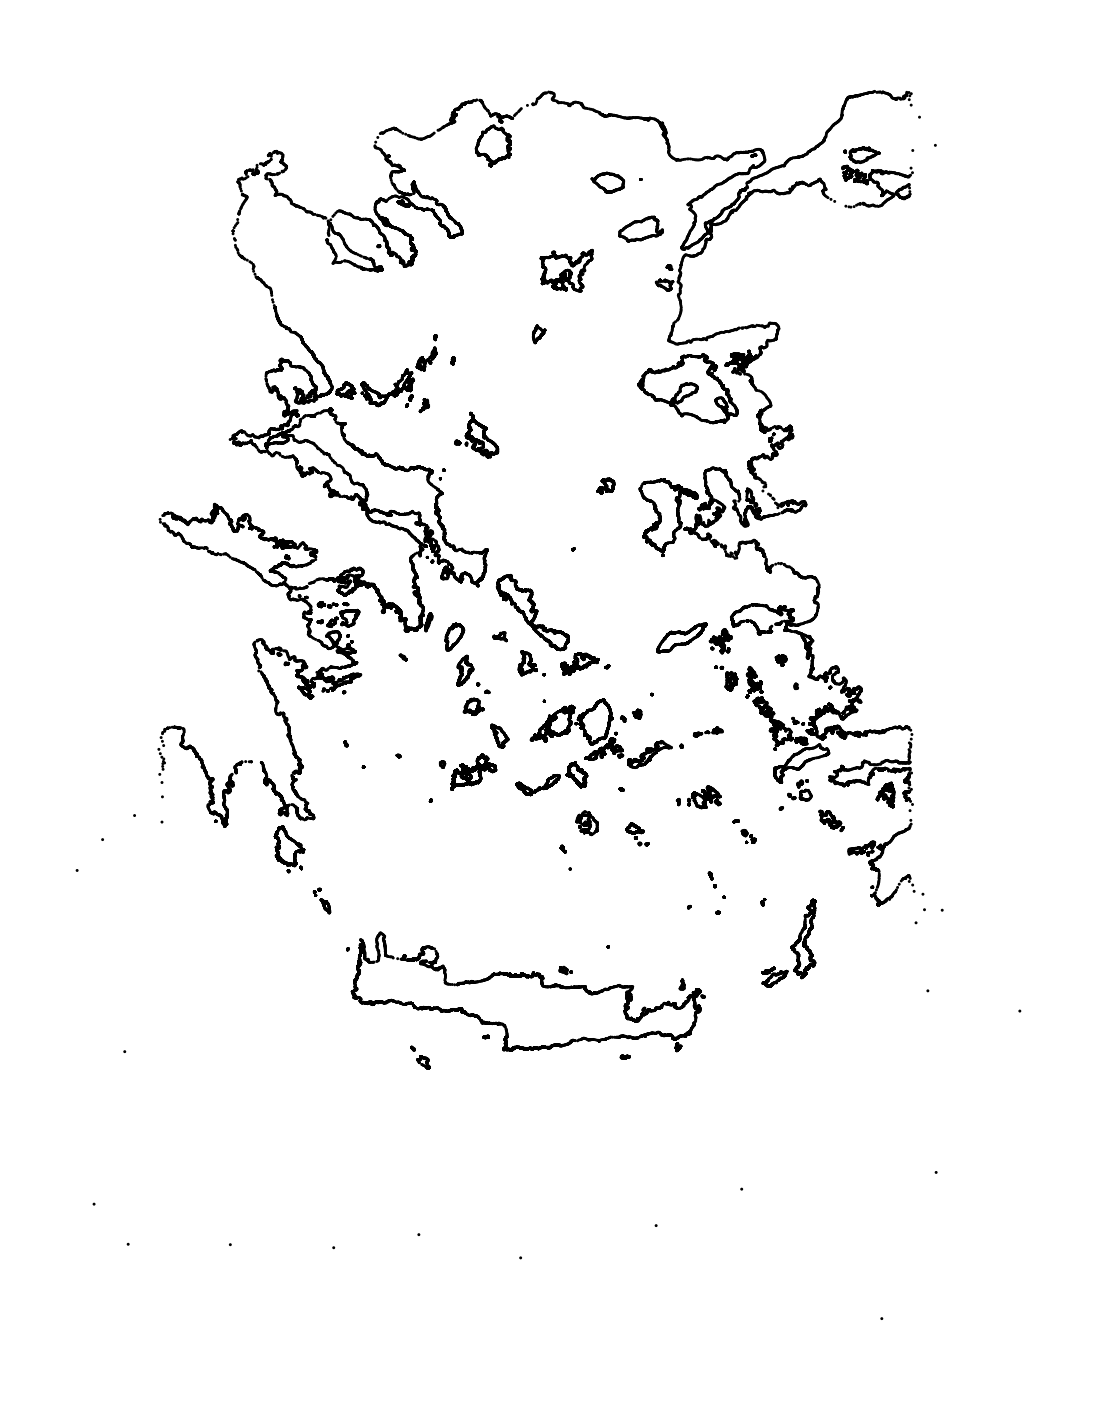
\includegraphics[width=\textwidth]{img/base_graphs/aegaeis-ref-visibility.png}
        \caption{aegaeis-visibility}
    \end{subfigure}
    \\
    \begin{subfigure}[b]{0.35\textwidth}
        \centering
        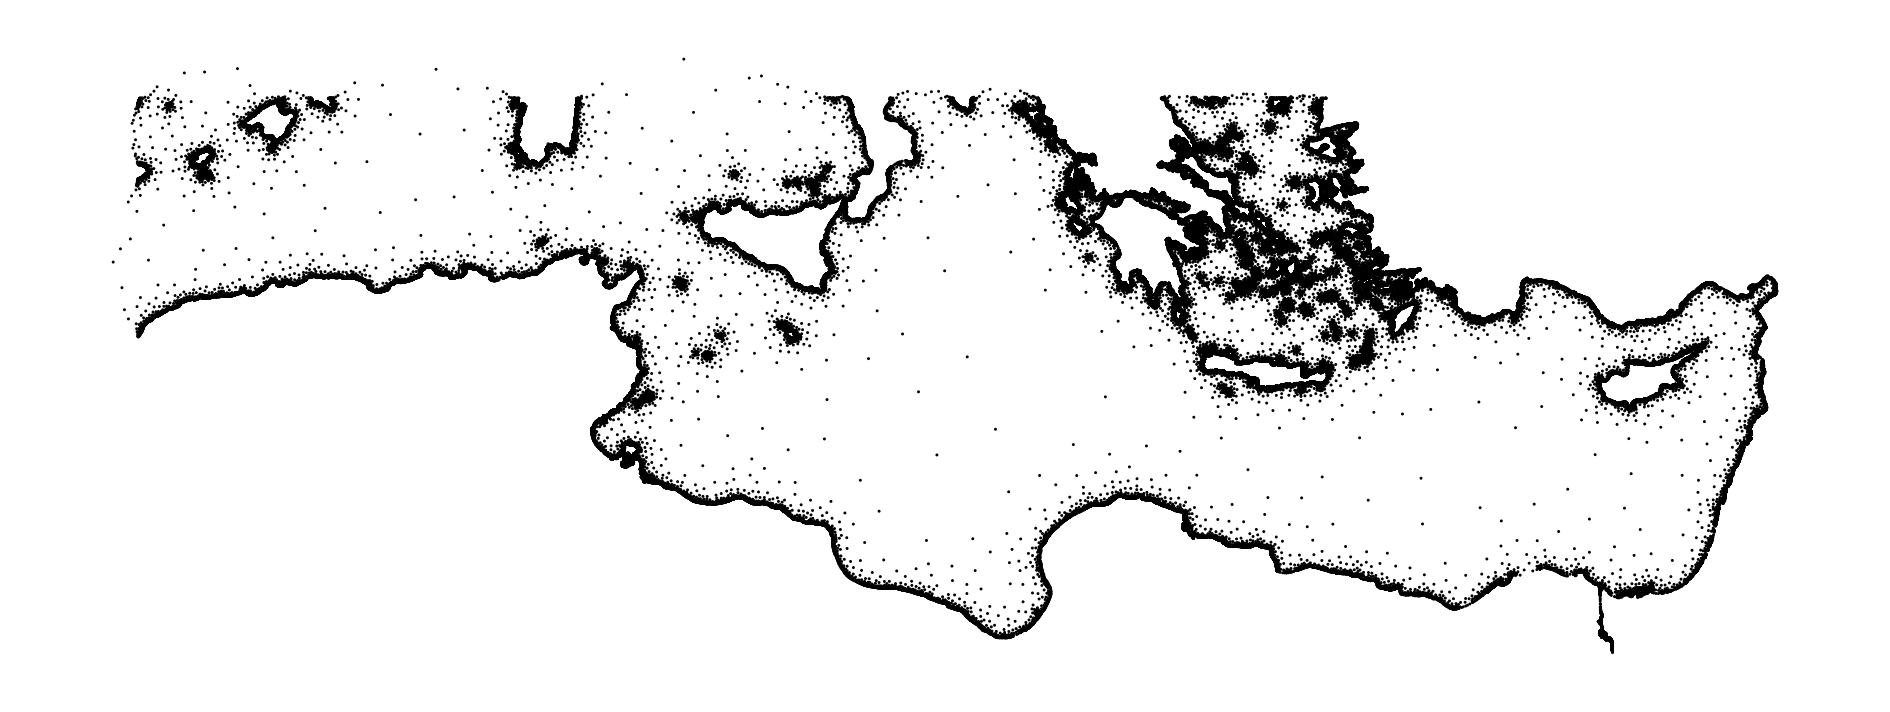
\includegraphics[width=\textwidth]{img/base_graphs/medi-ref-graph.png}
        \caption{medi-graph}
    \end{subfigure}
    \hfill
    \begin{subfigure}[b]{0.35\textwidth}
        \centering
        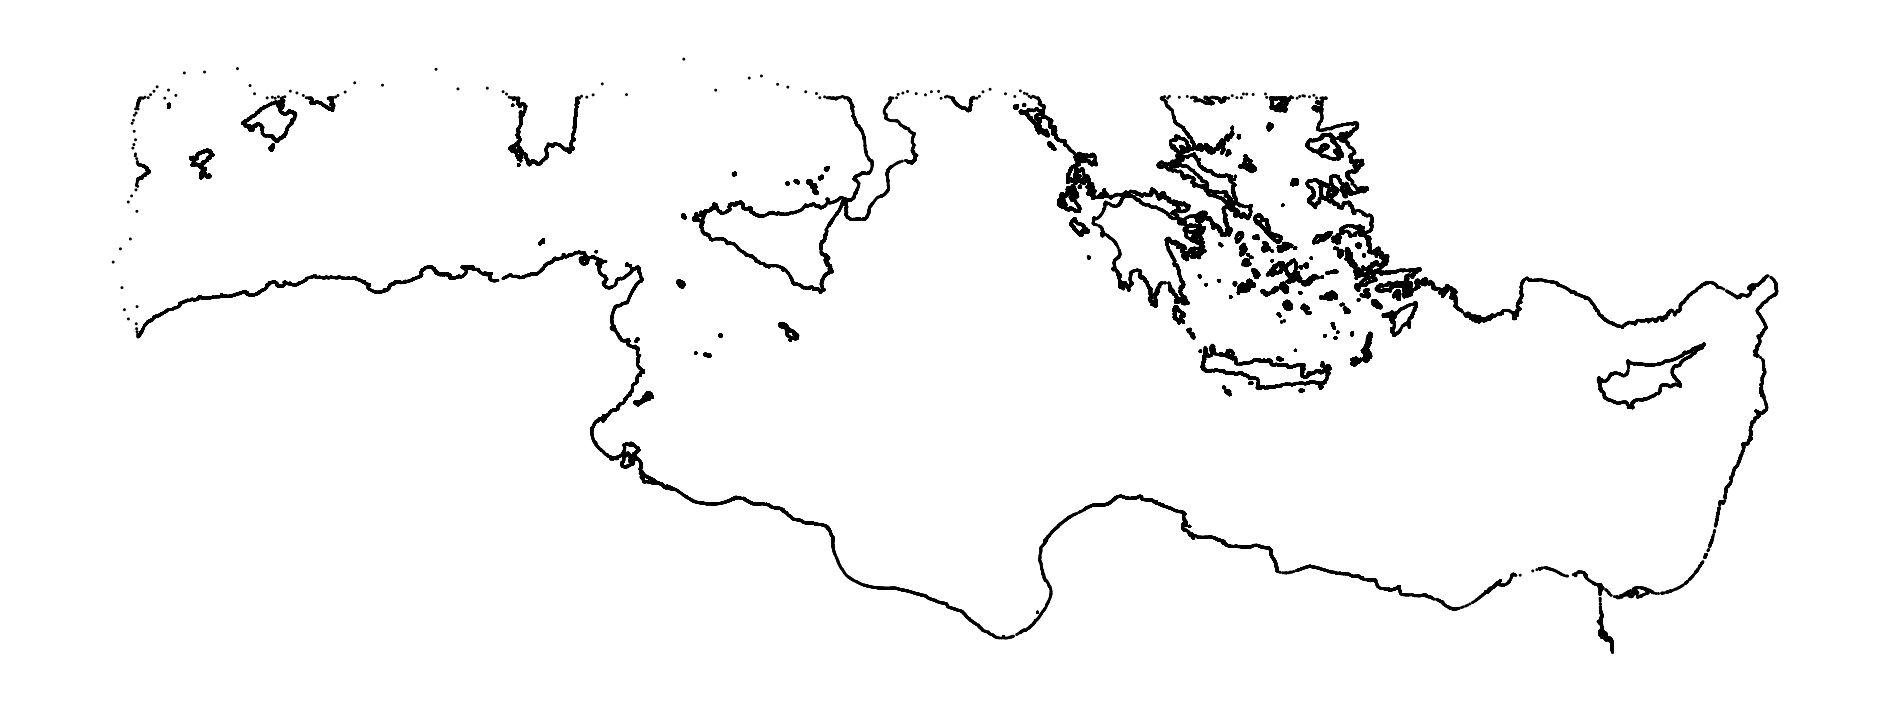
\includegraphics[width=\textwidth]{img/base_graphs/medi-ref-visibility.png}
        \caption{medi-visibility}
    \end{subfigure}
    \\
    \begin{subfigure}[b]{0.35\textwidth}
        \centering
        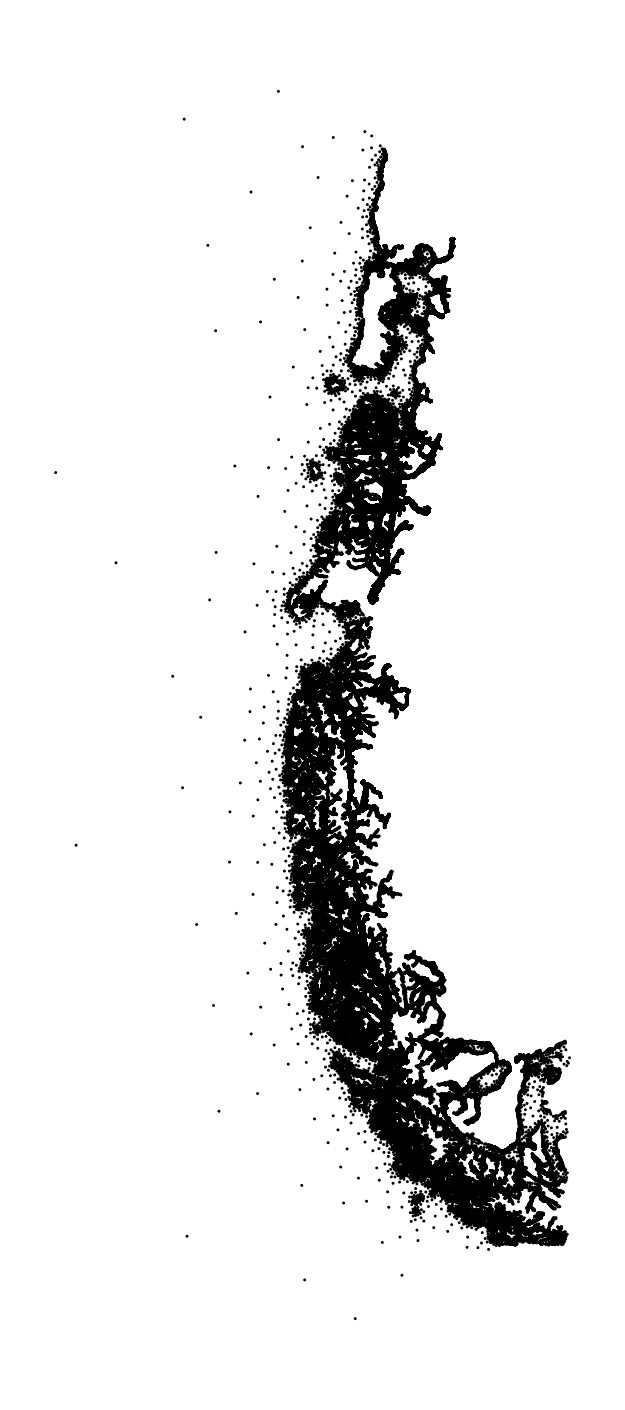
\includegraphics[width=\textwidth]{img/base_graphs/pata-ref-graph.png}
        \caption{pata-graph}
    \end{subfigure}
    \hfill
    \begin{subfigure}[b]{0.35\textwidth}
        \centering
        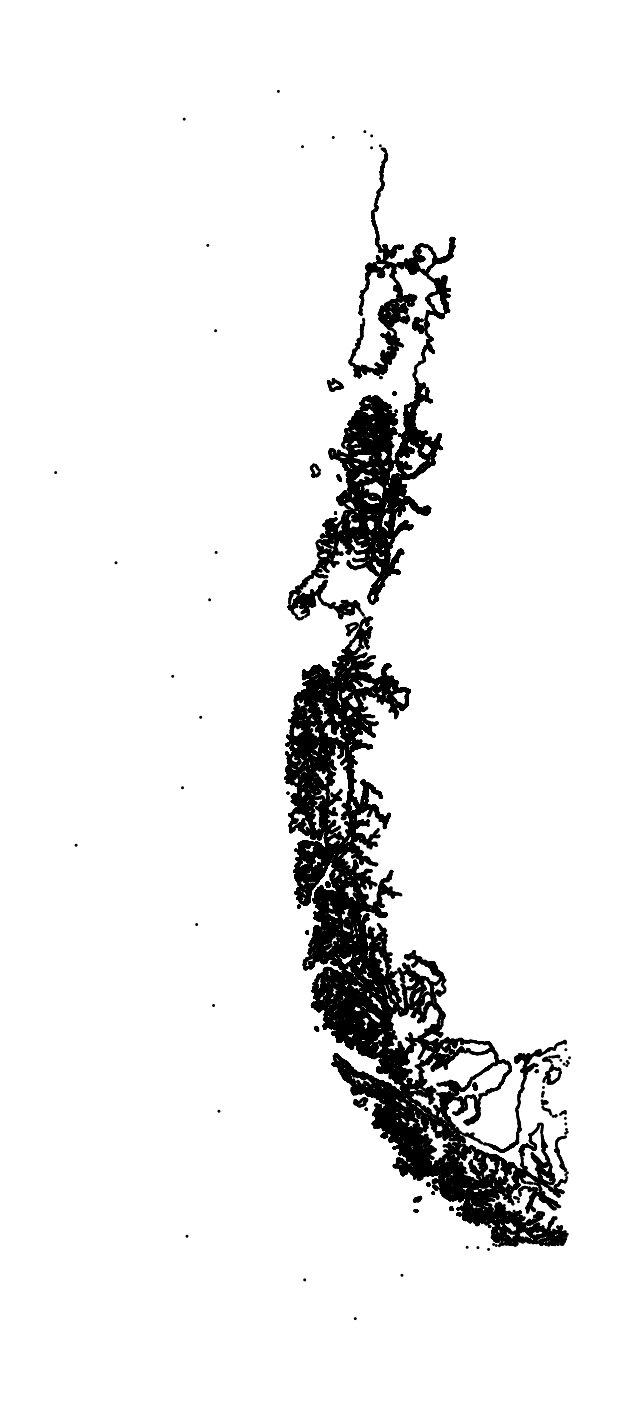
\includegraphics[width=\textwidth]{img/base_graphs/pata-ref-visibility.png}
        \caption{pata-visibility}
    \end{subfigure}
    \caption{Three simple graphs}
    \label{fig:three graphs}
\end{figure}


Sämtlichen Ergebisse wurden im BwUniCluster2.0 erzeugt. Sofern nicht anders erwähnt wurden
2x Intel Xeon Gold 6230
180GB RAM verwendet.


Die bereitgestellten Graphen mussten vor ihrer Nutzung gereinigt und an die Implementierung angepasst werden.
Sie enthielten isolierte Knoten, und die Kantengewichte der Sichtbarkeitsgraphen waren als Gleitkommazahlen gespeichert.
Für die Anpassung wurde ein Python-Skript benutzt, das folgende Aufgaben durchführt:

\begin{itemize}
    \item
          Transformation der Kantengewichte.

    \item
          Entfernung isolierter Knoten.

    \item
          Anpassung der Knoten-IDs, sodass die Knoten-IDs im Sichtbarkeitsgraphen den Bereich $0, \dotsc, n$ und im triangulierten Graphen den Bereich $0, \dotsc, n + m$ umfassen.
\end{itemize}

Während der Untersuchung der triangulierten Graphen wurde festgestellt, dass einige Kanten ein Gewicht von 0 aufwiesen.
Diese Kanten wurden unverändert beibehalten.

medi und pata Sichtbarkeitsgraphen fehlten jeweils einige Kanten, damit sie ungerichtet sind.
Diese wurden von Hand ergänzt.

\todo{Plot degree before after}

\section{Untersuchung der Graphen}

plot edge degree

vergleich der Abstände im vis und graph, sortiert nach hops in vis.




Vielleicht nur n mal insgesammt updaten? alle 10\% neu berechnen?



Heuristic egde difference (zufall)
Vis graphen haben sehr hohen degree (TODO Beweis).
Daher degree x degree viele checks, das gehtn schnell in die Millionen bis Milliarden.
Idee: betrachte nur ein Subset (tails, heads) und schaue ob und wie genau dieses die Edge difference aproximiert.

Das kann dann wieder für andere Methoden benutzt werden.

Plot hitting set vs bottom-up order

\section{Dijkstra}

Als Baseline wurden für jeden Graphen 1000 one-to-one Dijsktra-Suchen squentiell asugeführt. \todo{Darf ich auch parallel}?
Zur Speicherung der Distanzen und Vorgänger wurde ein Vec, als Warteschlange ein BinaryHeap und zum speichern, ob ein Knoten bereits expanded wurde ein BitSet verwendet.
\autoref{ergebnisse::table:dijkstra_one_to_one} zeigt die erzielten Zeiten.
Soweit nicht anders angegeben beziehen sich die Zeit immer auf das finden und erstellen des kürzesten Pfades.

\begin{table}[h]
    \centering
    \begin{tabular}{
            l % Graph
            S[table-format = 4.1] % Zeit
        }
        \toprule
        {Graph}            & {$\varnothing$ t (ms)} \\ \midrule
        aegaeis-graph      & 55.927509              \\
        aegaeis-visibility & 611.561878             \\
        medi-graph         & 93.091061              \\
        medi-visibility    & 1328.95972             \\
        pata-graph         & 245.354415             \\
        pata-visibility    & 964.165614             \\ \bottomrule
    \end{tabular}
    \caption{Dijkstra one-to-one, averaged over 1000 sequential searches}
    \label{ergebnisse::table:dijkstra_one_to_one}
\end{table}

Zusätzlich wurde die Durschnitliche Hop-Länge, Dijsktra Rank und Queue Pops untersucht.

\begin{table}[h]
    \centering
    \begin{tabular}{
            l % Graph
            S[table-format = 3.1] % hop-länge
            S[table-format = 7.0] % rank
            S[table-format = 7.0] % queue pops
        }
        \toprule
        {Graph}            & {Hop-Länge} & {Rank}    & {Queue pops} \\ \midrule
        aegaeis-graph      & 215.7201    & 260447.36 & 325845.56    \\
        aegaeis-visibility & 16.311      & 98650.82  & 517346.63    \\
        medi-graph         & 340.445     & 394855.78 & 494553.97    \\
        medi-visibility    & 23.6149     & 154092.42 & 959206.4     \\
        pata-graph         & 883.979     & 1120841.9 & 1387047.8    \\
        pata-visibility    & 63.817      & 498570.2  & 2429689.8    \\ \bottomrule
    \end{tabular}
    \caption{Dijkstra one-to-one, averaged over 1000 sequential searches}
\end{table}


Es wurde untersucht, ob es sinvoll ist, andere Datenstrukturen zu verwenden, insbesondere eine Warteschlange, die eine \emph{Drecrease-Key} Funktion anbietet.

\section{CH mit Witness}

Es wurde versucht die CH mit Witness, Edge Difference, Lacy Popping zu erstellen.
Dies hat für die Sichtbarkeitsgraphen nicht funktioniert, da 3 Tage nicht ausreichten die Graphen zu erzeugen.
Die Suche ist einfach zu teuer.
Pro Vorgänger muss eine Suche zu allen Nachfolgern gemacht werden.
\todo{Wie teuer ist das in der Ausgangslage?}

\begin{table}[h]
    \centering
    \begin{tabular}{
            l % Graph
            S[table-format = 1.2] % creation zeit
            S[table-format = 4.1] % average time
        }
        \toprule
        {Graph}       & {creation time (min)} & {$\varnothing$ t (µs)} \\ \midrule
        aegaeis-graph & 2.1336                & 514.069                \\
        medi-graph    & 3.08033333333         & 543.803                \\
        pata-graph    & 9.84055               & 730.317                \\\bottomrule
    \end{tabular}
    \caption{ch one-to-one, averaged over 1000 sequential searches}
\end{table}

\section{CH All-In}

All in sortiert nach all in edge differnce:


\section{Hitting Set}

Für die Graphen wurden jeweils ein Hitting Set über \num{100000} Pfade erstellt.
Diese Pfade wurden mit Dijkstra erstellt.

Wie hitbar sind die Graphen? plote hit percentage

\section{CH Bruteforce}

\begin{table}[h]
    \centering
    \begin{tabular}{
            l % Graph
            S[table-format = 1.2] % creation zeit
            S[table-format = 4.1] % average time
        }
        \toprule
        {Graph}            & {creation time (min)} & {$\varnothing$ t (µs)} \\ \midrule
        aegaeis-graph      &                       &                        \\
        aegaeis-visibility &                       &                        \\
        medi-graph         &                       &                        \\
        medi-visibility    &                       &                        \\
        pata-graph         &                       &                        \\
        pata-visibility    &                       &                        \\  \bottomrule
    \end{tabular}
    \caption{ch one-to-one, averaged over 1000 sequential searches}
\end{table}

\section{HL Merge}

Das Merging war deutlicht teruer als erwartet, da ch Kantengrad x HL Label Size

\begin{table}[h]
    \centering
    \begin{tabular}{
            l % Graph
            S[table-format = 1.2] % creation zeit
            S[table-format = 4.1] % average time
        }
        \toprule
        {Graph}            & {creation time (min)} & {$\varnothing$ t (µs)} \\ \midrule
        aegaeis-graph      &                       &                        \\
        aegaeis-visibility &                       &                        \\
        medi-graph         &                       &                        \\
        medi-visibility    &                       &                        \\
        pata-graph         &                       &                        \\
        pata-visibility    &                       &                        \\  \bottomrule
    \end{tabular}
    \caption{hl one-to-one, averaged over 1000 sequential searches}
\end{table}

\section{HL Bruteforce}

\begin{table}[h]
    \centering
    \begin{tabular}{
            l % Graph
            S[table-format = 1.2] % creation zeit
            S[table-format = 4.1] % average time
        }
        \toprule
        {Graph}            & {creation time (min)} & {$\varnothing$ t (µs)} \\ \midrule
        aegaeis-graph      &                       &                        \\
        aegaeis-visibility &                       &                        \\
        medi-graph         &                       &                        \\
        medi-visibility    &                       &                        \\
        pata-graph         &                       &                        \\
        pata-visibility    &                       &                        \\  \bottomrule
    \end{tabular}
    \caption{hl one-to-one, averaged over 1000 sequential searches}
\end{table}

\section{Großes Hitting set}

\section{}
